\documentclass[a4paper,12pt]{article}
\usepackage[english]{babel}
\usepackage[utf8]{inputenc}

%
% For alternative styles, see the biblatex manual:
% http://mirrors.ctan.org/macros/latex/contrib/biblatex/doc/biblatex.pdf
%
% The 'verbose' family of styles produces full citations in footnotes, 
% with and a variety of options for ibidem abbreviations.
%
\usepackage{graphicx}
\usepackage{csquotes}
\usepackage[style=verbose-ibid,backend=bibtex]{biblatex}
\bibliography{sample}

\usepackage{lipsum} % for dummy text

\title{Linear Least-Squares Algorithms for Temporal Difference Learning}

\author{Shayan Amani}

\date{\today}

\begin{document}
\maketitle

\section{Intro}
prediction of overall reward during a span of time can be calculated by applying TD algorithms to the system. According to what the authors pointed out and showed later, the two introduced algorithms can yield more details out of training process of the understudied system, However, they may not be that computationally-wise efficient compared to Sutton's $TD(\lambda)$. 

\section{Markov Decision Processes}
In this paper an \textit{infinite-horizon} \textit{finite-state} \textit{discounted-reward} Markov Decision Process has been examined. Finding an optimal \textbf{fixed} policy according to its definition by applying\textbf{ policy iteration} method.

\section{Least-Squares in TD Learning}
Combining computational efficiency of TD learning methods with the power of least-squares methods in terms of fast reaching to a desired accuracy can bring up another approach to this type of problems, namely least-squares temporal difference method. It's better to have it in mind that, least-squares algorithms often take less time step in comparison to temporal difference algorithms to reach the desired accuracy.

\section{Introduced Methods}
The authors proposed three methods derived from temporal difference algorithm:
\begin{itemize}
    \item $NTD(\lambda)$: normalized temporal difference method $TD(\lambda)$.
    \item LS TD: probing value function using Least-Squares theorem.
    \item RLS TD: approaching the LS TD's desired accuracy in a recursive manner.
\end{itemize}

\section{Error Variance of a Markov Chain}
As the author proposed, the error variance for a temporal difference learning method ($\sigma_{TD}$) is defined by the noise of the algorithm itself. Again as we can see in below, convergence time has a direct relationship with $\sigma_{TD}$:

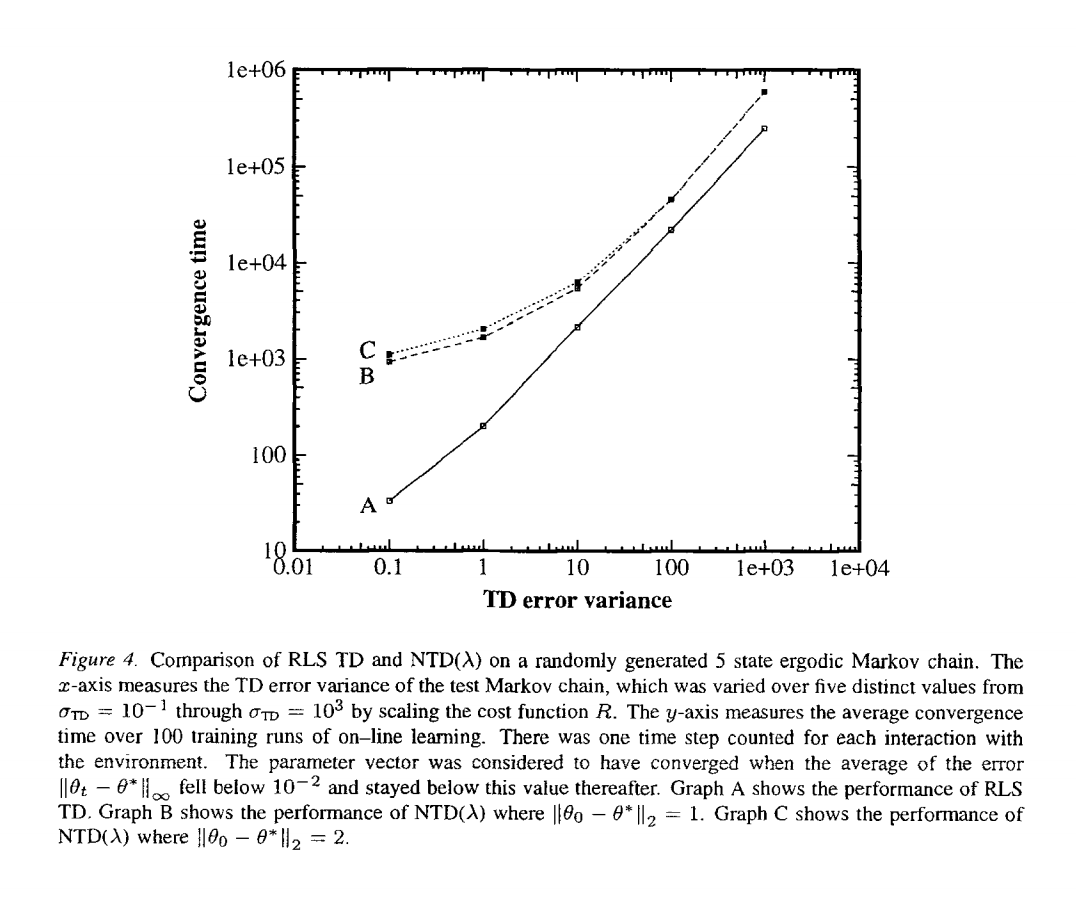
\includegraphics[width=1\columnwidth]{fig4-error-var.png}

\section{Questions}
\subsection{How is LSTD relate to TD (temporal difference)?}
According to what discussed earlier, LSTD take advantage of the approximation power of  Least-Squares method in order to probe a value function. Technically speaking, linear-in-the-parameters approximator in conjunction with the regular temporal difference algorithm facilitates calculation of $\theta^*$.

\subsection{When will TD and LSTD solutions be the same?}
I assume that if we can observe a linear behaviour among the problem components such as transition probability function and reward, so we can expect to get a same solution from Linear-Squares TD and the regular TD. Although the approach that we take in LSTD to solve the problem may differ than TD but if we have a problem with liear properties, so approximating with LS technique could not emerge with big difference in the final solution.

% This is an example citation \autocite{ginsberg}.
% \lipsum[1] % dummy text

% This is another example citation \autocite{brassard}.
% \lipsum[2] % dummy text

% This is a repeated citation \autocite{brassard}.
% \lipsum[3] % dummy text

% This is another example citation \autocite{adorf}.
% \lipsum[4] % dummy text 

\end{document}